\documentclass{article}

\usepackage{siunitx} % Provides the \SI{}{} and \si{} command for typesetting SI units
\usepackage{graphicx} % Required for the inclusion of images
\usepackage{epstopdf}
\usepackage{natbib} % Required to change bibliography style to APA
\usepackage{amsmath} % Required for some math elements 
\usepackage{amsmath}
\usepackage{verbatim}
\usepackage{hyperref}
\usepackage{tikz}
\usetikzlibrary{matrix}

\tikzstyle{block} = [draw, rectangle, minimum height=2em, minimum width=4em]

\setlength\parindent{0pt} % Removes all indentation from paragraphs

\renewcommand{\labelenumi}{\alph{enumi}.} 

\renewcommand{\c}[1]{\cos(\theta_{#1})}
\newcommand{\s}[1]{\sin(\theta_{#1})}
\newcommand{\T}[2]{{}^{#1}T_{#2}}
\renewcommand{\O}[2]{{}^{#1}O_{#2}}

\title{Robots Fundamentals:\\
Assignment report} % Title

\author{Rodrigo \textsc{Moreno Carrillo} \\
			Mang \textsc{Ning}} % Author name

\date{\today} % Date for the report 
\begin{document}
%call:

\maketitle % Insert the title, author and date

\section{Part 1}
\subsection{Forward kinematics} 

According with the diagram of the Lynxmotion robot depicted in figure $\ref{fig:forward.diagram}$ the corresponding Denavit-Harterverg table based on distal convention is:

\begin{table}[h!]
\centering
\begin{tabular}{ c | c c c c}
 n & $a_n$ 	& $\alpha_n$		& $d_n$	& $\theta_n$\\ \hline
 1 & 0 			& 90º				& $d_1$	& $\theta_1$\\  
 2 & $a_2$ 	& 0					& 0			& $\theta_2$\\  
 3 & $a_3$ 	& 0					& 0			& $\theta_3$\\  
 4 & 0 			& 90º				& 0			& $\theta_4$\\  
 5 & 0 			& 0					& $d_5$	& $\theta_5$\\ 
\end{tabular}
\caption{Denavit-Hartenverg table using distal convention}
\label{tab:forward.dh}
\end{table}

The robot contains five different reference frames which are described by the parameters in table \ref{tab:forward.dh}. Correspondingly, the homogeneous transformation between frames can be described as below:

\begin{equation}
\label{eq:forward.t_01}
\T{0}{1} = \left[
\begin{array}{cccc}
	\c{1} & 0 & \s{1} & 0 \\
	\s{1} & 0 & -\c{1} & 0 \\
	0 & 1 & 0 & d_1 \\
	0 & 0 & 0 & 1 \\
\end{array}
\right]
\end{equation}

\begin{equation}
\label{eq:forward.t_12}
\T{1}{2} =\left[
\begin{array}{cccc}
	\c{2} & -\s{2} & 0 & a_2\c{2} \\
	\s{2} & \c{2} & 0 & a_2\s{2}  \\
	0 & 0 & 1 & 0 \\
	0 & 0 & 0 & 1 \\
\end{array}
\right]
\end{equation}

\begin{equation}
\label{eq:forward.t_23}
\T{2}{3} =\left[
\begin{array}{cccc}
	\c{3} & -\s{3} & 0 & a_3\c{3} \\
	\s{3} & \c{3} & 0 & a_3\s{3}  \\
	0 & 0 & 1 & 0 \\
	0 & 0 & 0 & 1 \\
\end{array}
\right]
\end{equation}

\begin{equation}
\label{eq:forward.t_34}
\T{3}{4} = \left[
\begin{array}{cccc}
	\c{4} & 0 & \s{4} & 0 \\
	\s{4} & 0 & -\c{4} & 0 \\
	0 & 1 & 0 & 0 \\
	0 & 0 & 0 & 1 \\
\end{array}
\right]
\end{equation}

\begin{equation}
\label{eq:forward.t_45}
\T{4}{5} =\left[
\begin{array}{cccc}
	\c{5} & -\s{5} & 0 & 0 \\
	\s{5} & \c{5} & 0 & 0  \\
	0 & 0 & 1 & d_5\\
	0 & 0 & 0 & 1 \\
\end{array}
\right]
\end{equation}

where $a_2 = 9.5$ [cm], $a_3 = 11$ [cm], $d_1 = 6.5$ [cm] and $d_5 = 3.2$ [cm].

\begin{figure}[htbp]
\begin{center}
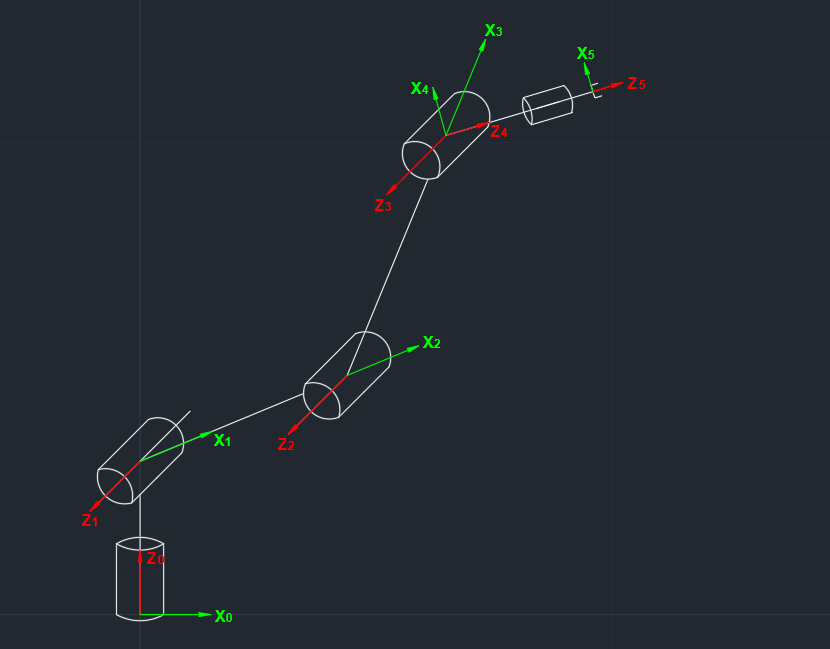
\includegraphics[width=0.8\textwidth]{images/diagram}
\caption{Lynxmotion robot diagram}
\label{fig:forward.diagram}
\end{center}
\end{figure}

The forward kinematics consists of knowing the orientation and position of the end effector with respect to the world frame whose origin is at point $O_0$. According to the rule of matrix multiplication, $\T{0}{5}$ describes what is needed and it can be derived from

\begin{equation}
\T{0}{5} = \T{0}{1} \T{1}{2}\T{2}{3}\T{3}{4}\T{4}{5}
\end{equation}

Thus, the resultant matrix will be a homogeneous matrix that represents the orientation and position of the frame attached at the end effector. It will depend on the variables $\theta_1 ... \theta_5$ and have the following form:

\begin{subequations}
\begin{align}
\T{0}{5} & = \left[
\begin{array}{cccc}
	r_{11} & r_{12} & r_{13} & {}^0Ox_5 \\
	r_{21} & r_{22} & r_{23} & {}^0Oy_5 \\
	r_{31} & r_{32} & r_{33} & {}^0Oz_5 \\
	0 & 0 & 0 & 1 \\
\end{array}
\right] \\
& = \left[
\begin{array}{cc}
	R & {}^0O_5 \\
	 0 & 1 \\
\end{array}
\right] 
\end{align}
\end{subequations}

where $R$ is the rotation matrix of the fifth frame and ${}^0O_5$ is the coordinate vector of point $O_5$ with respect to the world frame. ${}^0O_5$  is also the desired point of the end effector.

\begin{equation*}
{}^0O_5 = \left[
\begin{array}{c}
	{}^0Ox_5 \\
	{}^0Oy_5 \\
	{}^0Oz_5 \\
\end{array}
\right] = \left[
\begin{array}{c}
	{}^0P_x \\
	{}^0P_y \\
	{}^0P_z \\
\end{array}
\right] = {}^0P
\end{equation*}

To compute the forward kinematics in Matlab, a function is created to receive the vector $Q=[\theta_1 \theta_2 \theta_3 \theta_4 \theta_5]^T$ as input and output the position ${}^0P$ and orientation $R$ of the end effector, which is depicted in figure \ref{fig:forward.block_diagram}.

\begin{figure}[htbp] 
\begin{center}
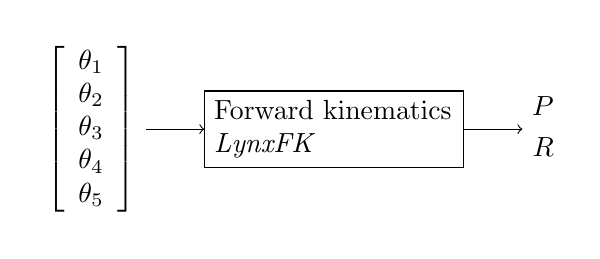
\begin{tikzpicture}
	\matrix [ row sep = .375cm, column sep = .75cm, ]
	{
	\node (Q_INPUT) {$\left[ \begin{array}{c}
	\theta_1 \\
	\theta_2 \\
	\theta_3 \\
	\theta_4 \\
	\theta_5 \\ \end{array} \right]$}; &
	\node (FK) [block]{\parbox[c]{1.2in}{Forward kinematics \\ \textit{LynxFK}}}; &
	\node (PR_OUTPUT) {$\begin{aligned}P\\R\end{aligned}$}; \\};
	\draw[->](Q_INPUT)-{}(FK);
	\draw[->](FK)-{}(PR_OUTPUT);
\end{tikzpicture}
\caption{Forward kinematics diagram}
\label{fig:forward.block_diagram}
\end{center}
\end{figure}

\subsection{Workspace}
The operational range of every joint variales $\theta_i$ is necessary for tracing out the workspace.  The relevant parameters are in table \ref{tab:workspace.range}.

\begin{table}[h!]
\centering
\begin{tabular}{ c | c }
Variable		& Operational range [º]\\ \hline
$\theta_1$	& [-90, 90]\\
$\theta_2$	& [0, 135]\\
$\theta_3$	& [-135, 30]\\
$\theta_4$	& [0, 180]\\
$\theta_5$	& [-90, 90]
\end{tabular}
\caption{Operational range of joint variables}
\label{tab:workspace.range}
\end{table}

Once the range of the variables has been determined, the movement of every joint can be simulated to create a reachable 3D space for the end effector, figure \ref{fig:workpace.workspace} presents the workspace. Specifically, the top left picture shows a 3D space, while the others intuitively present a 2D view in the planes of YX, ZX and ZY respectively.

\begin{figure}[htbp]
\begin{center}
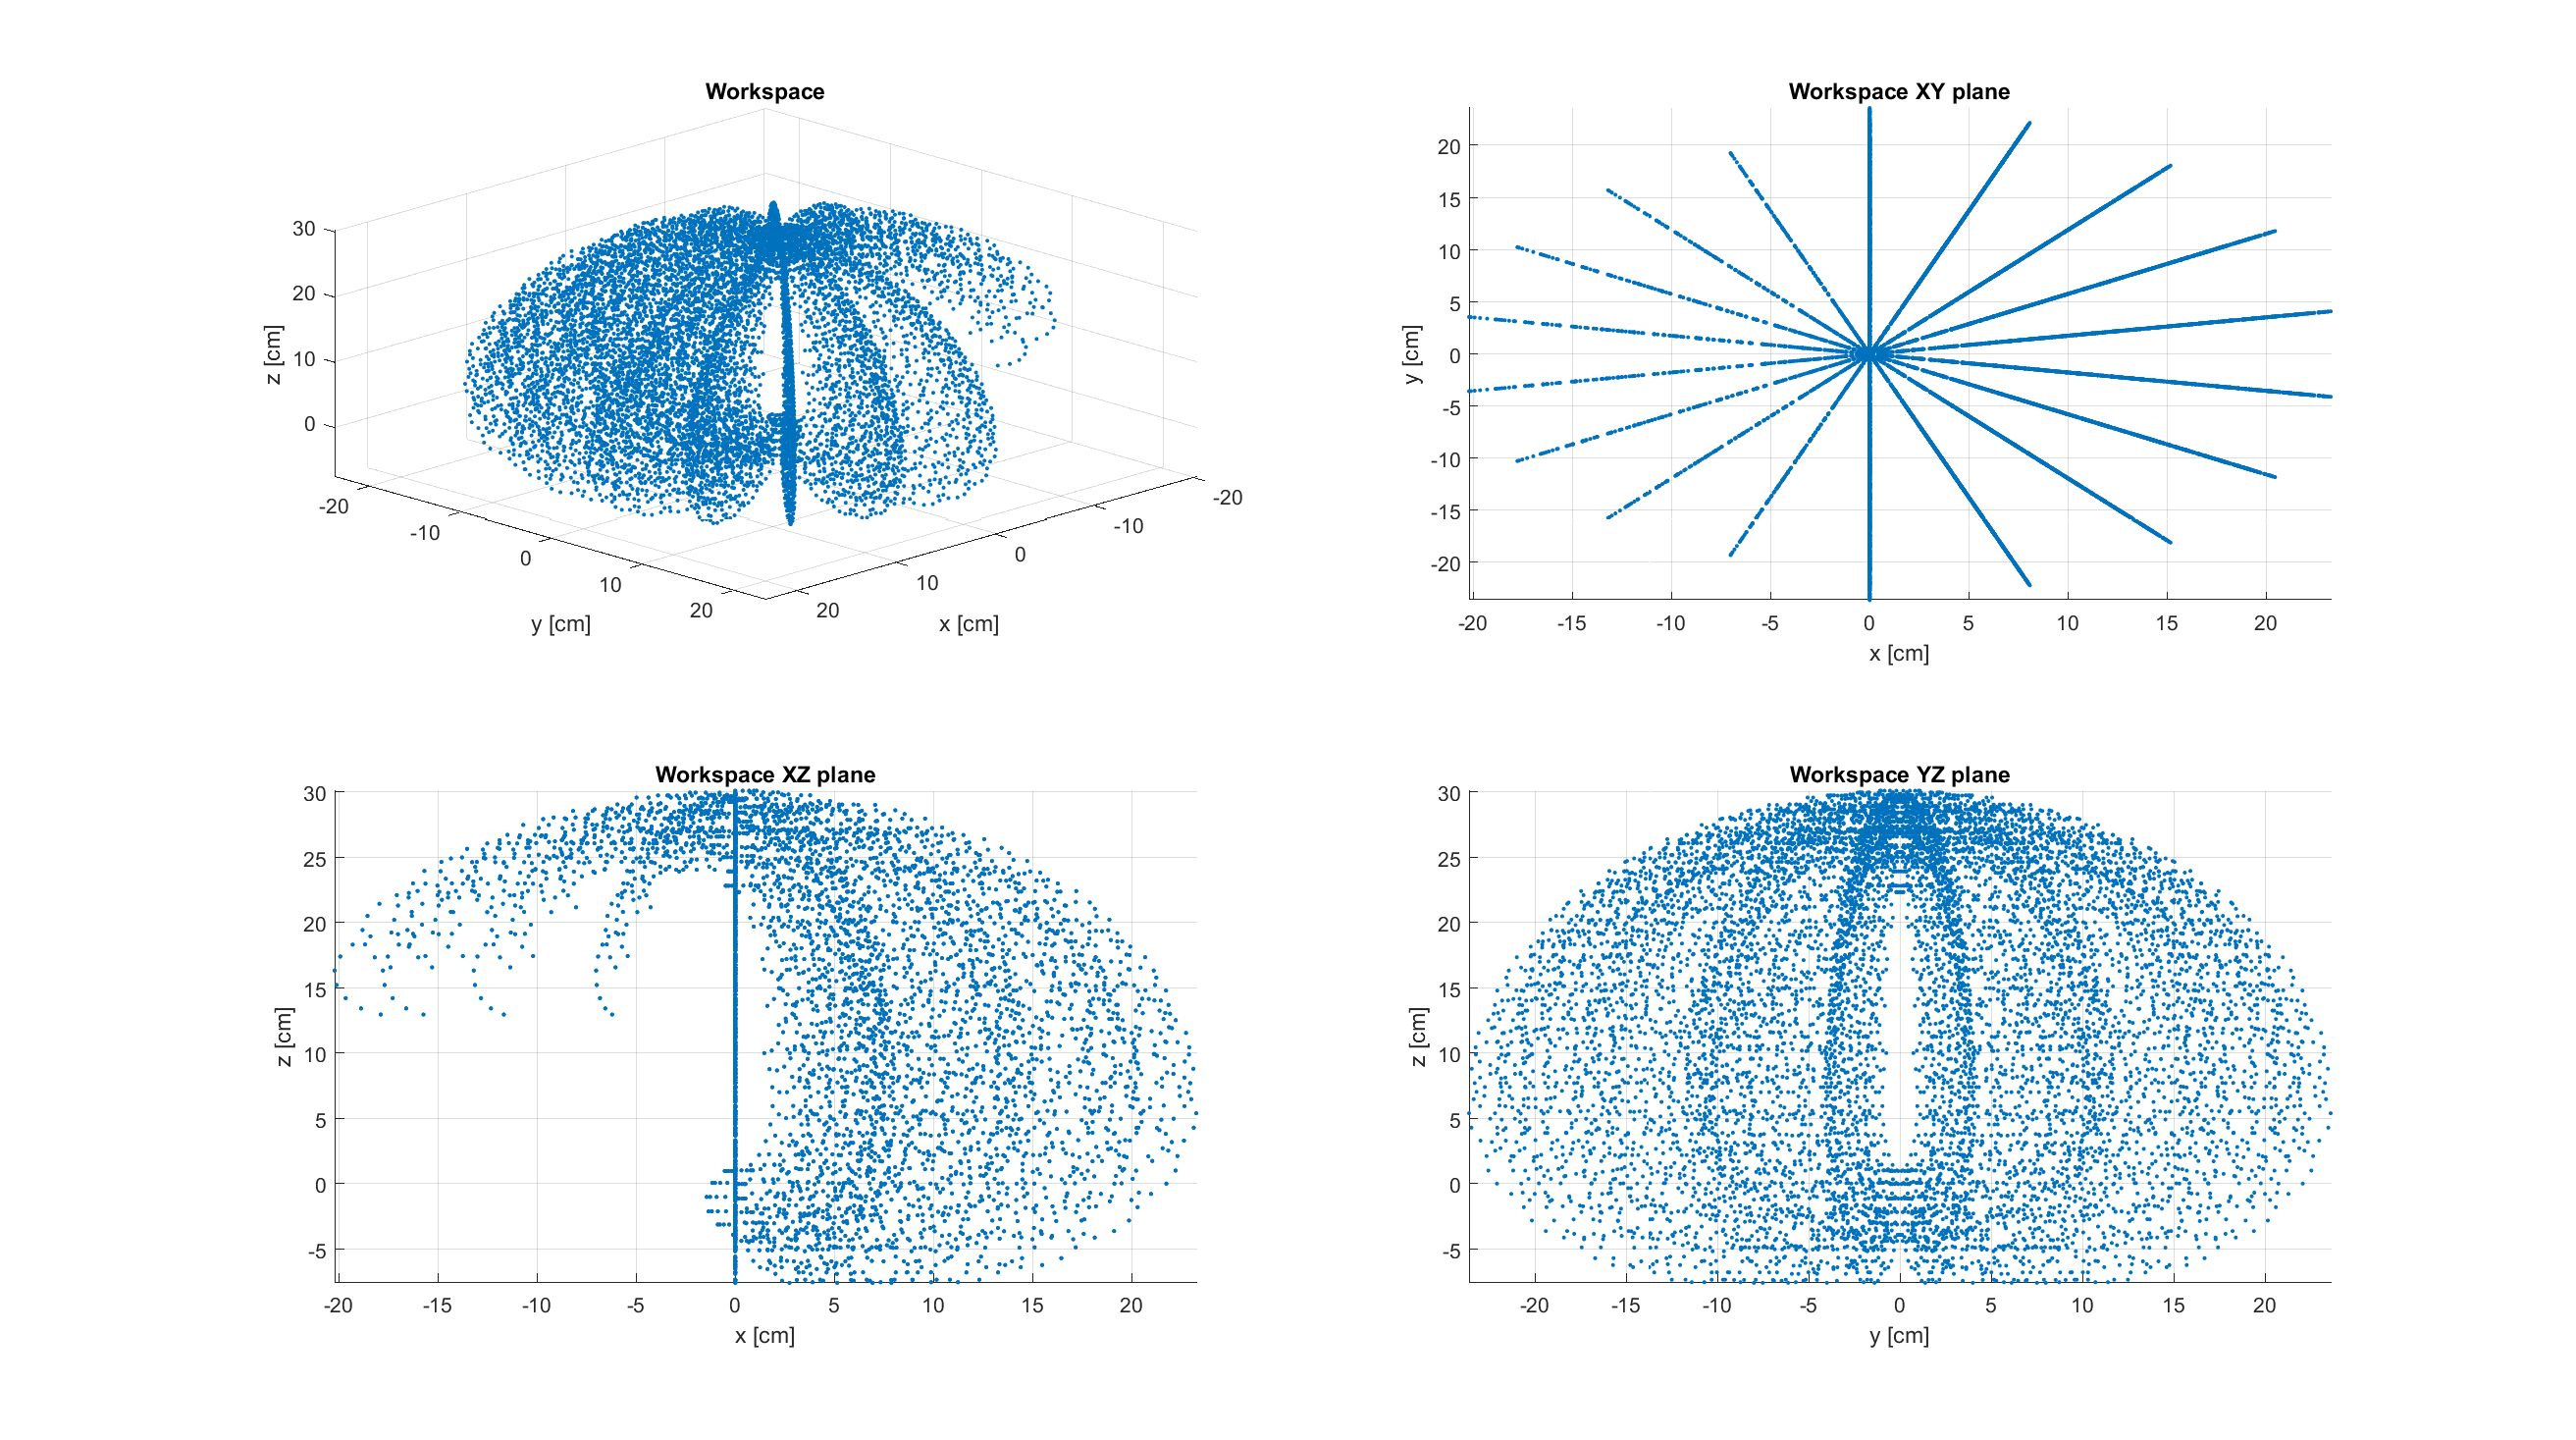
\includegraphics[width=\textwidth]{images/Workspace}
\caption{Lynxmotion robot workspace}
\label{fig:workpace.workspace}
\end{center}
\end{figure}

\subsection{Inverse kinematics}
The purpose of inverse kinematics is to find the joint valuables given the specific position and orientation of the end effector. Concretely, there are five joints valuables need to be worked out, namely  $\theta_1$,  $\theta_2$,  $\theta_3$,  $\theta_4$,  $\theta_5$.

\subsubsection{Finding  $\theta_1$}
Since the x and y position of the end effector are only decided by the rotation of joint 1, we can project the manipulator into the horizontal plane of the world frame. Therefore, we can derive the expression of  $\theta_1$

\begin{equation}
\theta_1 = atan2(Py, Px)
\end{equation}

\subsubsection{Finding  $\theta_2$, $\theta_3$}
For simplifying the configuration, we can extract link 2 and link 3 from the whole manipulator, hence the link 2 and link 3 would be a planar mechanism. The next step is to find the origin coordinates of frame 3 regarding frame 1, namely $\O{1}{3}$, which can be derived from the matrix of $\T{1}{3}$. Furthermore, $\T{1}{3}$ can be expressed as the product

\begin{align}
\label{eq:inverse.t_13}
\T{0}{1}\T{1}{3} & = \T{0}{3} \nonumber \\
{(\T{0}{1})}^{-1}\T{0}{1}\T{1}{3}& = {(\T{0}{1})}^{-1} \T{0}{3} \nonumber \\
\T{1}{3} & = \T{1}{0} \T{0}{3}
\end{align}

According to the equation (\ref{eq:inverse.t_13}), we need to get the matrixes $\T{1}{0}$ and $\T{0}{3}$ respectively. $\T{1}{0}$ is easy to get from the inverse matrix of $\T{0}{1}$, which should be 

\begin{equation}
\label{eq:inverse.t_10}
{(\T{0}{1})}^{-1} = \T{1}{0} = \left[
\begin{array}{cccc}
	\c{1} & \s{1} & 0 & 0 \\
	0 & 0 & 1 & -d_1 \\
	\s{1} & -\c{1} & 0 & 0 \\
	0 & 0 & 0 & 1 \\
\end{array}
\right]
\end{equation}

As for  $\T{0}{3}$, we only focus on the displacement part $\O{0}{3}$(the last column of $\T{0}{3}$).

\begin{equation}
\label{eq:inverse.t_03}
\T{0}{3} = \left[ \begin{array}{cccc}
	\cdot & \cdot & \cdot & {}^0O_{3x} \\
	\cdot & \cdot & \cdot & {}^0O_{3y} \\
	\cdot & \cdot & \cdot & {}^0O_{3z} \\
	0 & 0 & 0 & 1 \\
\end{array} \right]
\end{equation}

Furthermore, $Z_5$ is aligned with link 4 whose length is $d_5$, so $\O{0}{3}$ can be calculated by

\begin{equation}
\label{eq:inverse.O_03}
\begin{aligned}
\O{0}{3} & = {}^0P - d_5 R\left[
\begin{array}{c}
	0 \\
	0 \\
	1 \\
\end{array} \right]  \\
\left[
\begin{array}{c}
	{}^0O_{3x} \\
	{}^0O_{3y} \\
	{}^0O_{3z} \\
\end{array} \right] & = \left[
\begin{array}{c}
	{}^0P_x \\
	{}^0P_y \\
	{}^0P_z \\
\end{array}
\right] - d_5 \left[ \begin{array}{c}
	{}r_{13} \\
	{}r_{23} \\
	{}r_{33} \\
\end{array} \right]
\end{aligned}
\end{equation}

Then, $\T{1}{3}$ can be computed by substituting (\ref{eq:inverse.t_10}), (\ref{eq:inverse.t_03}) and (\ref{eq:inverse.O_03}) in (\ref{eq:inverse.t_13}). Lastly, as only the fourth column is needed at this moment, equation (\ref{eq:inverse.t_13_expanded}) only shows the last column for simplicity.

\begin{equation}
\label{eq:inverse.t_13_expanded}
\T{1}{3} = \left[ \begin{array}{cccc}
	\cdot & \cdot & \cdot & \O{0}{3x} \c{1} + \O{0}{3y} \s{1} \\
	\cdot & \cdot & \cdot & \O{0}{3z}-d_1 \\
	\cdot & \cdot & \cdot & \O{0}{3x} \s{1}-\O{0}{3y} \c{1} \\
	0 & 0 & 0 & 1 \\
\end{array} \right]
\end{equation}

Therefore, we found the coordinates of frame 3 with respect to frame 1(namely $\O{1}{3}$), as denoted in equation (\ref{eq:inverse.O_13}). Then the solutions of  $\theta_2$ and  $\theta_3$ can be worked out by the geometrical method mentioned in the lecture. There are 2 solutions as a result of redundancy, which is shown below in figure \ref{fig:theta_2,theta_3}.

\begin{align}
\label{eq:inverse.O_13}
\O{1}{3} = 
\left[ \begin{array}{c}
	\O{1}{3x} \\
	\O{1}{3y} \\
	\O{1}{3z} \\
\end{array} \right] = \left[ \begin{array}{c}
	\O{0}{3x} \c{1} + \O{0}{3y} \s{1} \\
	\O{0}{3z}-d_1 \\
	\O{0}{3x} \s{1}-\O{0}{3y} \c{1} \\
\end{array} \right]
\end{align}

\begin{figure}[htbp] 
\begin{center}
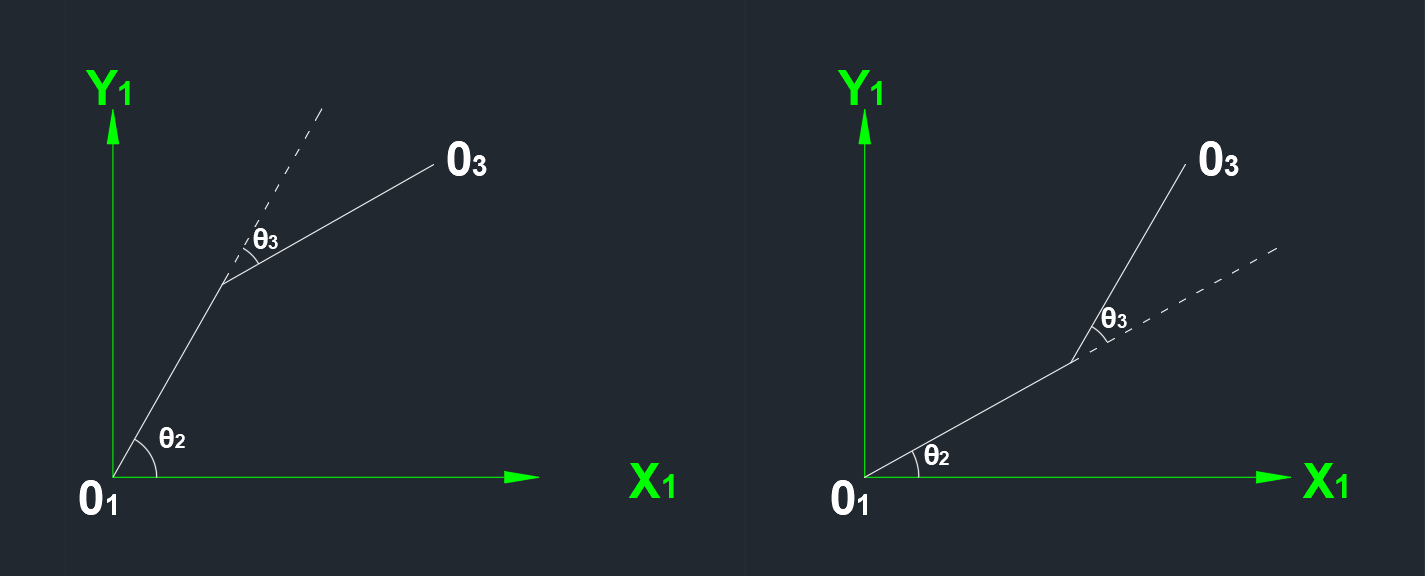
\includegraphics[width=\textwidth]{images/theta2,theta3}
\caption{Graphical representation of the two solutions for $\theta_2$ and $\theta_3$, namely elbow left and elbow right}
\label{fig:theta_2,theta_3}
\end{center}
\end{figure}

Applying the law of cosines and using the coordinates of point $O_3$ with respect to $O_1$, we can derive the expression of $\theta_3$ that
\begin{equation*}
\c{3} = \frac{\O{1}{3x}^2 + \O{1}{3y}^2 - a_2^2 - a_3^2}{2a_2a_3}\qquad
\end{equation*}
while sine will have two possible values, a positive and a negative value, which will lead to the two solutions depicted above.
\begin{equation*}
\s{3} = \pm\sqrt{1-\c{3}^2}
\end{equation*}

\begin{equation*}
\theta_{3} = \begin{cases} 
   \theta_{3_1} & \text{for } {\s{3}}^+ \\
   \theta_{3_2} & \text{for } {\s{3}}^-
  \end{cases}
\end{equation*}

\begin{equation}
\theta_{3} = atan2(\s{3},\c{3})
\end{equation}

Finally, $\theta_2$ can be computed from the angle of $\O{1}{3}$ once that $\theta_3$ is known.

\begin{equation}
\theta_{2} = atan2(\O{1}{3y},\O{1}{3x})-atan2(\sin(b),\cos(b) )
\end{equation}
where
\begin{equation*}
\sin(b)= \frac{a_3\s{3}}{\sqrt{\O{1}{3x}^2+\O{1}{3y}^2}}
\end{equation*}

Due to the dependence of $\theta_2$ and $\theta_3$,  $\theta_2$ will also have two solutions. The two sets of solutions create two possible configurations, elbow right for $\theta_3^+$ and elbow left for $\theta_3^-$, which are depicted in figure \ref{fig:theta_2,theta_3}.

\subsubsection{Finding $\theta_4$}
The algebraic method is used to work out $\theta_4$. The core idea is building an equation of $\theta_4$ from the element of transformation matrix $\T{3}{5}$.Now,$\theta_1$, $\theta_2$, $\theta_3$ are already known. Combined with  $\T{0}{5}$,  $\T{3}{5}$ can be derived from

\begin{align}
\label{eq:inverse.t_35}
\T{0}{3}\T{3}{5} & = \T{0}{5} \nonumber \\
{(\T{0}{3})}^{-1}\T{0}{3}\T{3}{5}& = {(\T{0}{3})}^{-1} \T{0}{5} \nonumber \\
\T{3}{5} & = \T{3}{0} \T{0}{5}
\end{align}

where

\begin{equation}
\label{eq:inverse.t_30}
\T{3}{0} = \T{3}{2}\T{2}{1}\T{1}{0} 
\end{equation}

Each element on the right side of equation \ref{eq:inverse.t_35} depends on $\theta_1$, $\theta_2$ and $\theta_3$ which are already known. It is vital to mention that there exists two versions of $\T{3}{2}$ and $\T{2}{1}$ as there are two solutions. Therefore, $\T{3}{5}$ will have two versions and both have the form:

\begin{equation}
\label{eq:inverse.t_35_expanded}
\T{3}{5}= \left[
\begin{array}{cccc}
	\cdot & \cdot & \cdot & \O{3}{5x} \\
	\cdot & \cdot & \cdot & \O{3}{5y} \\
	\cdot & \cdot & \cdot & \O{3}{5z} \\
    0 & 0 & 0 & 1 \\
\end{array}
\right] 
\end{equation}

Another way to get $\T{3}{5}$ with variable $\theta_4$ is multiplying matrix (\ref{eq:forward.t_34}) and matrix (\ref{eq:forward.t_45}).

\begin{equation}
\begin{aligned}
\label{eq:inverse.t_35_forward}
\T{3}{5} = \T{3}{4} \T{4}{5} & =
\left[
\begin{array}{cccc}
	\c{4} & 0 & \s{4} & 0 \\
	\s{4} & 0 & -\c{4} & 0 \\
	0 & 1 & 0 & 0 \\
	0 & 0 & 0 & 1 \\
\end{array}
\right] \left[
\begin{array}{cccc}
	\c{5} & -\s{5} & 0 & 0 \\
	\s{5} & \c{5} & 0 & 0  \\
	0 & 0 & 1 & d_5\\
	0 & 0 & 0 & 1 \\
\end{array}
\right] \\
& = \left[
\begin{array}{cccc}
	\cdot & \cdot & \cdot & d_5\s{4} \\
	\cdot & \cdot & \cdot & -d_5\c{4}\\
	\cdot & \cdot & \cdot & 0\\
    0 & 0 & 0 & 1 \\
\end{array}
\right] 
\end{aligned}
\end{equation}

Thus, $\T{3}{5}$ has been derived in two ways, which can be used to create an equation system to solve for $\theta_4$. By equalising the last column of (\ref{eq:inverse.t_35_expanded}) and (\ref{eq:inverse.t_35_forward}) we obtain:

\begin{equation}
\s{4} = \frac{\O{3}{5x}}{d_5}
\qquad
\c{4} = -\frac{\O{3}{5y}}{d_5}
\end{equation}
therefore
\begin{equation}
\theta_{4} = atan2(\s{4},\c{4})
\end{equation}

As a result of the two versions of (\ref{eq:inverse.t_35_expanded}), $\theta_4$ will also have two solutions that must be computed in the same way for both configurations.

\subsubsection{Finding $\theta_5$}
The method of calculating $\theta_5$ is similar to finding $\theta_4$. we try to get the matrix  $\T{4}{5}$ from two ways. The one with variable $\theta_5$ is obviously expressed in equation \ref{eq:forward.t_45}.

Another means of representing $\T{4}{5}$ is 
\begin{equation}
\label{eq:inverse.t_45}
\T{4}{5} = \T{4}{0} \T{0}{5}
\end{equation}
where
\begin{equation*}
\T{4}{0} = \T{4}{3}\T{3}{0}
\end{equation*}
consequently, the equation (\ref{eq:inverse.t_45}) depends on the inverse of (\ref{eq:forward.t_34}), (\ref{eq:inverse.t_03}) since $\T{0}{5}$ is a known condition. 

It seems that $\theta_5$ should also have two solutions since $\s{4}$ and $\c{4}$ have 2 pairs of solutions and the expression of $\T{4}{0}$ contains $\s{4}$ and $\c{4}$. Whereas, it turns out that $\T{4}{0}$ only have one value due to the same computing result of 2 pairs of $\s{4}$ and $\c{4}$.For simplicity, (a,b) is used to represent each element of $\T{4}{5}$(a,b are the numble of rows and columns). so, $\s{5}$ and $\c{5}$ can be written as

\begin{equation}
\s{5} = \T{4}{5}(2,1)
\qquad
\c{5} = \T{4}{5}(1,1)
\end{equation}
Hence,the solutions of $\theta_5$ is
\begin{equation}
\theta_{5} = atan2(\s{5},\c{5})
\end{equation}

\subsection{Task plan}
The chosen task is to simulate the process of picking three objects and stick them on a wall. In this case the robot should take an object and move it to the target position, then repeat this operation for the remaining twe objects.

These points are chosen inside the workspace, the detail can be seen in the figure \ref{fig:points.points}.

\begin{figure}
\begin{center}
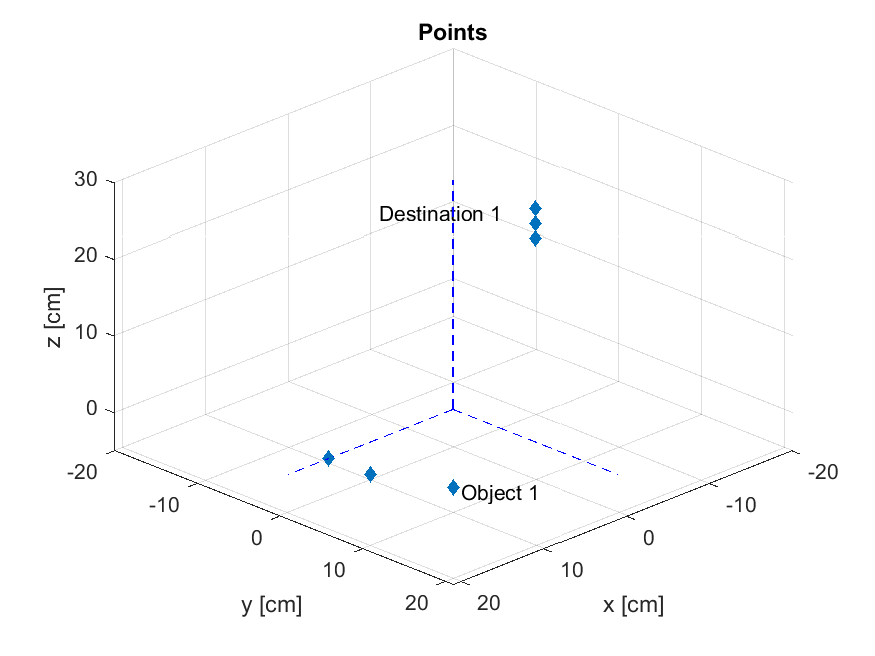
\includegraphics[width=\textwidth]{images/Points}
\caption{Chosen points for the pick and place task}
\label{fig:points.points}
\end{center}
\end{figure}

\begin{figure}
\begin{center}
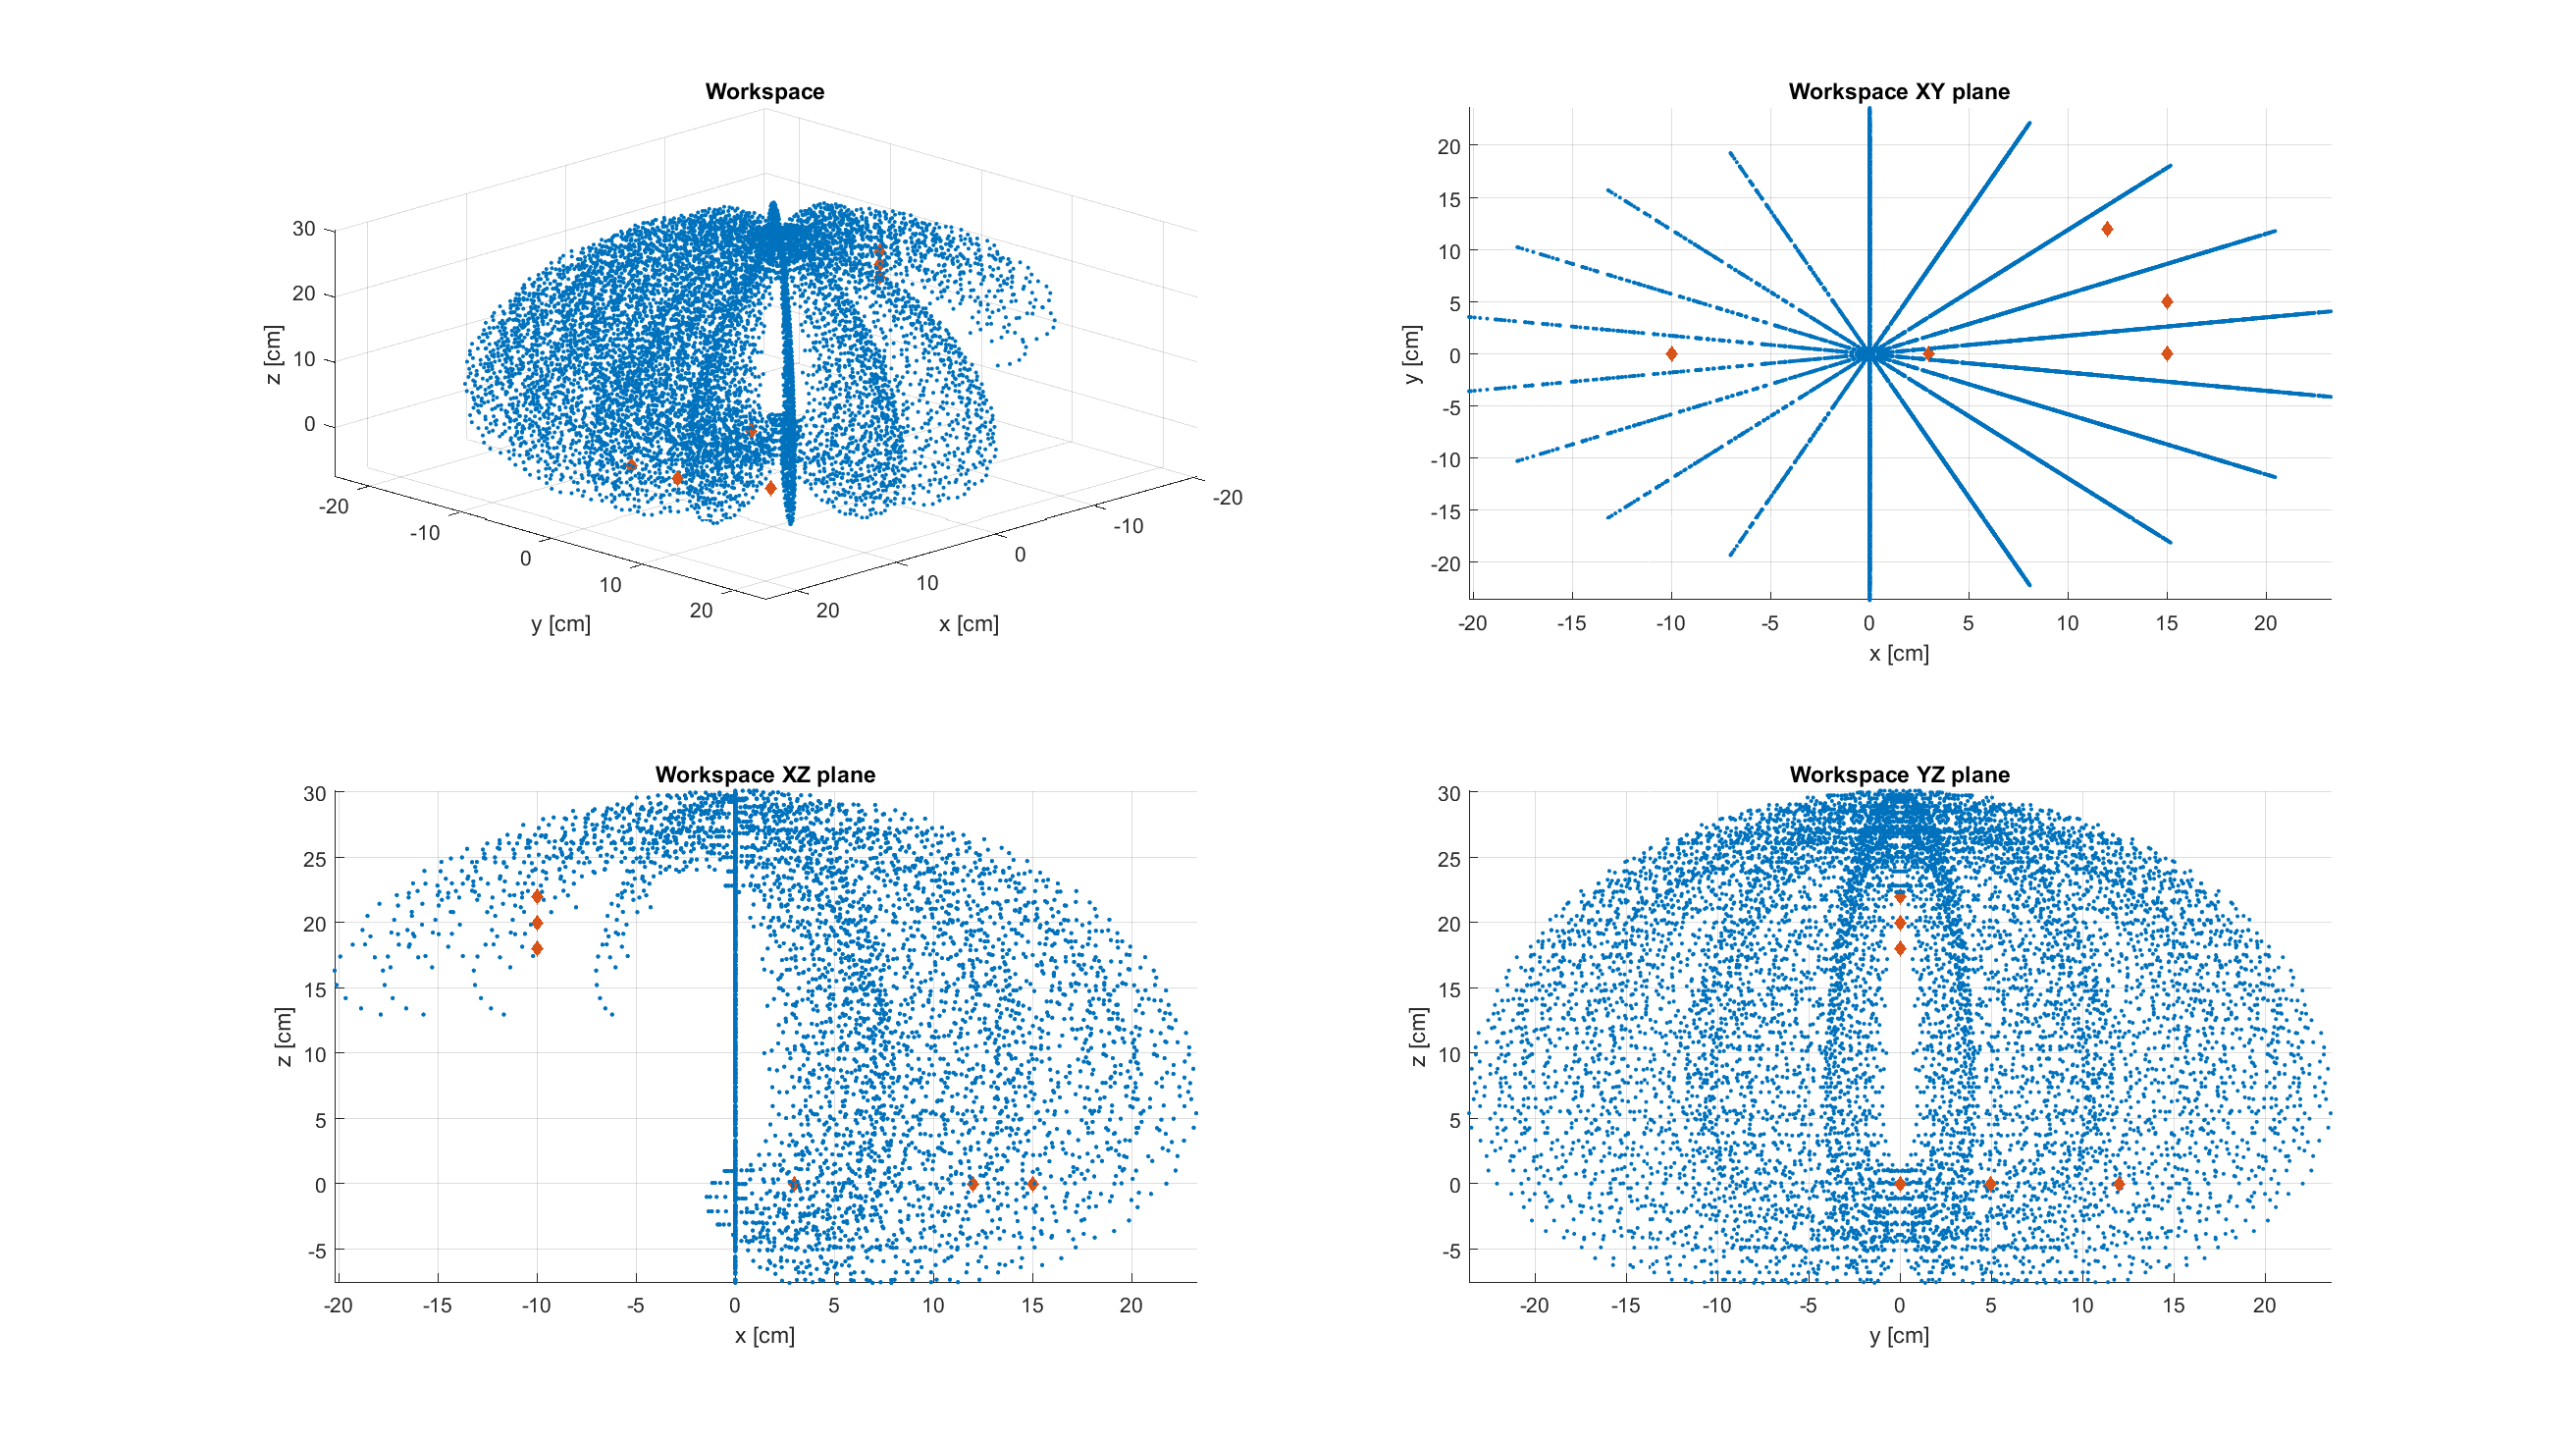
\includegraphics[width=\textwidth]{images/Workspace_Points}
\caption{Workspace and chosen points}
\label{fig:points.ws_points}
\end{center}
\end{figure}

\subsection{Forward kinematics test}

The aim of this section is to generate the position and the orientation parameters of the end effector for those selected six points above.

To execute the experiment,the \textit{LynxFK} function is created to take a set of joint values as input and output the corresponding orientation and position information for a particular robot configuration.

For convenience of subsequent inverse kinematics test, the outcomes of the forward kinematics test are saved into a file. 

\subsection{Inverse kinematics test and animation}
Inverse kinematics calcultes the set of joint values ($\theta_i^{\prime}$) through loading the pair data $P$ and $R$ which are stored in the previous files. Then, for validating the results of the inverse kinematics process, the robot will compute the forward kinematics using the given output which should produce a new set of points, called $P^{\prime}$ and $R^{\prime}$, which should be similar to those used as input for inverse kinematics. This process is depicted by figure \ref{fig:inverse_test.diagram}.

\begin{figure}
\begin{center}
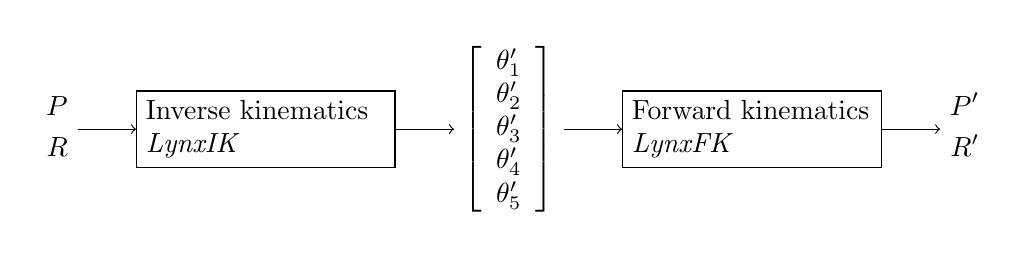
\begin{tikzpicture}
	\matrix [ row sep = .375cm, column sep = .75cm, ]
	{
	\node (PR_INPUT) {$\begin{aligned}P\\R\end{aligned}$}; &
	\node (IK) [block]{\parbox[c]{1.2in}{Inverse kinematics \\ \textit{LynxIK}}}; &
	\node (Q_OUTPUT) {$\left[ \begin{array}{c}
	\theta_1^{\prime} \\
	\theta_2^{\prime} \\
	\theta_3^{\prime} \\
	\theta_4^{\prime} \\
	\theta_5^{\prime} \\ \end{array} \right]$}; &
	\node (FK) [block]{\parbox[c]{1.2in}{Forward kinematics \\ \textit{LynxFK}}}; &
	\node (PR_OUTPUT) {$\begin{aligned}P^{\prime}\\R^{\prime}\end{aligned}$}; \\
	};
	
	\draw[->](PR_INPUT)-{}(IK);
	\draw[->](IK)-{}(Q_OUTPUT);
	\draw[->](Q_OUTPUT)-{}(FK);
	\draw[->](FK)-{}(PR_OUTPUT);
\end{tikzpicture}
\caption{Inverse kinematics diagram}
\label{fig:inverse_test.diagram}
\end{center}
\end{figure}

To provide a quantitative measure of the result, we use an error function $e_i$ to compute the difference between the desired position ($P$) and the obtained position ($P_i^{\prime}$) at the point $i$.  The results of the first solution are shown in table \ref{tab:inverse_test.error}.

\begin{equation}
e_i=P_i-P_i^{\prime}
\end{equation}

\begin{table}[h!]
\centering
\begin{tabular}{ c | c c c || c}
 $e_i$ 	& $e_x$ 		& $e_y$	& $e_z$		& $|e_i|$\\ \hline
 1 			& -0.7403 	& 0			& -0.8710		& 1.1432\\
 2 			& 0 				& 0			& 0				& 0\\ 
 3 			& 0 				& 0			& 0				& 0\\ 
 4 			& 0 				& 0			& 0				& 0\\ 
 5 			& 0 				& 0			& 0				& 0\\
 6 			& 0 				& 0			& 0				& 0\\
 7 			& 0 				& 0			& 0				& 0\\
\end{tabular}
\caption{Error of the resultant position, $e_i=P_i-P_i^{\prime}$}
\label{tab:inverse_test.error}
\end{table}

\begin{figure}
\begin{center}
\includegraphics[width=\textwidth]{images/inverse_test}
\caption{Workspace and chosen points}
\label{fig:inverse_test.test}
\end{center}
\end{figure}

\subsection{Trajectories}
All three of these trajectories have been accomplished and combined to achieve a single task, which will be elaborated in the following.
\subsubsection{Polynomial trajectories}
The via point approach is used to implement the desired trajectories to create the paths. Specifically, we compute the coefficients of the polynomials that best fit to those paths.

The considered polynomial trajectory is 4-3-4. This means the first and last trajectory is a polynomial of fourth degree whilst a polynomial of third degree is used for the inner trajectories .

\begin{equation}
q(t) = 
  \begin{cases} 
  q_1(t)= a_4t^4 + a_3t^3 + a_2t^2 + a_1t + a_0 & : t_0 \leq t < t_1 \\
   q_2(t)= b_3t^3 + b_2t^2 + b_1t + b_0 & : t_1 \leq t < t_2 \\
   q_3(t)= c_4t^4 + c_3t^3 + c_2t^2 + c_1t + c_0 & : t_2 \leq t < t_f
  \end{cases}
\end{equation}

Finally, we only need to calculate the values of the coefficients to fully describe the piecewise trajectory at the desired points.

\subsubsection{Straight line}
In order to implement an straight line between the chosen points it was created a line between them, using the parametric form of the equation of the line in 3D where the parameter in this case is the time, and uniformly sampled to get the via points that the robot should follow using the polynomial trajectory.

\begin{equation}
\mathbf{p}=\mathbf{u}t + \mathbf{p_0}
\end{equation}

Where, $\mathbf{p}$, $\mathbf{u}$, $\mathbf{p_0}$ $\in R^3$. If the times at every chosen point is known, the direction vector $\mathbf{u}$ and point $\mathbf{p_0}$ can be computed therefore the line can be sampled giving the position along the line that connect the desired points as a function of time. 

For this case the orientation was considered to be constant so the position and the orientation is known and by performing the inverse kinematics for every sample on the line a trajectory can be computed using the first and last point as starting and ending point respectively and the inner points as via points using the approach described previously.

\subsubsection{Object avoidance}
For the object avoidance requirement, the approach used to compute the trajectory that avoid a collision with an an obstacle consist in sampling a straight line in the same way as before but once the sampled points are known the next step is to relocate them in order to avoid the obstacle.

\begin{equation}
\label{eq:trajectories.displacement}
\mathbf{d}=\frac{R_k}{||\mathbf{r}||^2}\frac{\mathbf{r}}{||\mathbf{r}||}
\end{equation}

To relocate the points the equation \ref{eq:trajectories.displacement} was used to compute the displacement, where $\mathbf{r}$ is the vector from the obstacle to a via point, $R_k$ is a repulsive constant and $d$ is displacement vector. Later the displacement is added to the analysed point to get the new position.

\begin{equation}
\mathbf{p}^{\prime}=\mathbf{p}+\mathbf{d}
\end{equation}

In figure \ref{fig:trajectories.cartesian} it can be observed that the obstacle modify the last trajectory due to the relocation of the via points.

\begin{figure}
\begin{center}
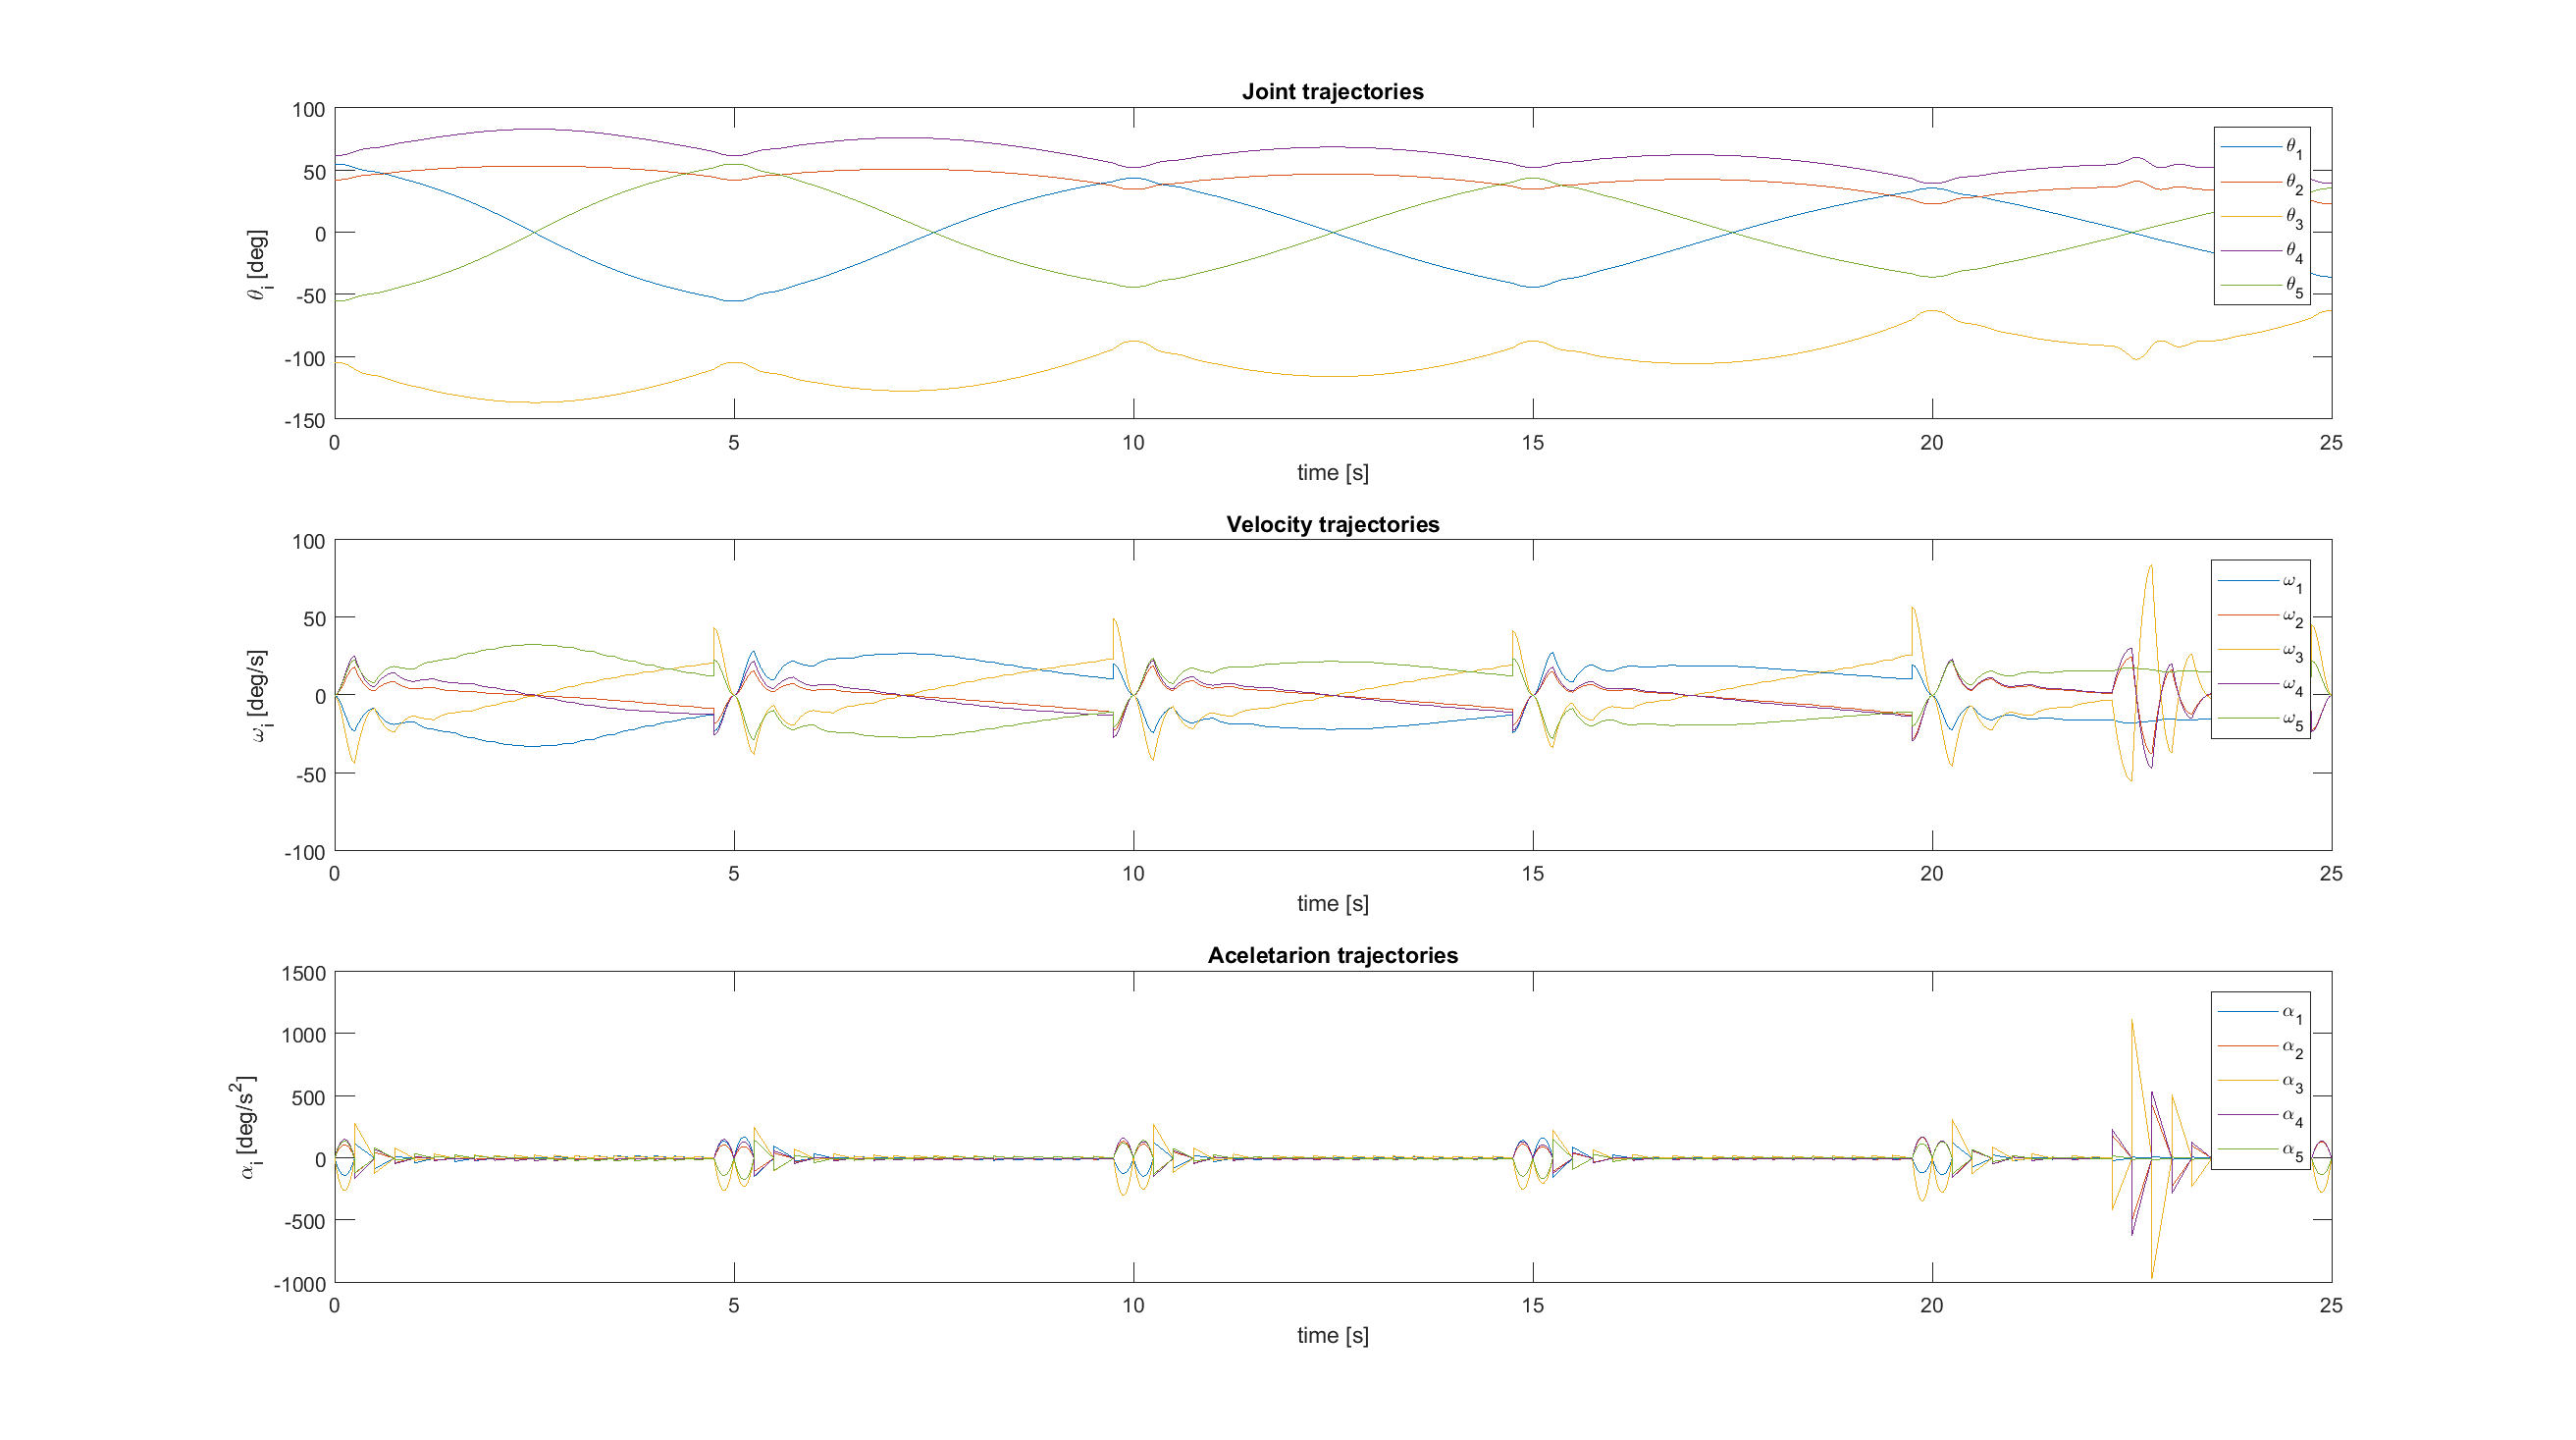
\includegraphics[width=\textwidth]{images/Trajectory_Joint}
\caption{Workspace and chosen points}
\label{fig:trajectories.joints}
\end{center}
\end{figure}

\begin{figure}
\begin{center}
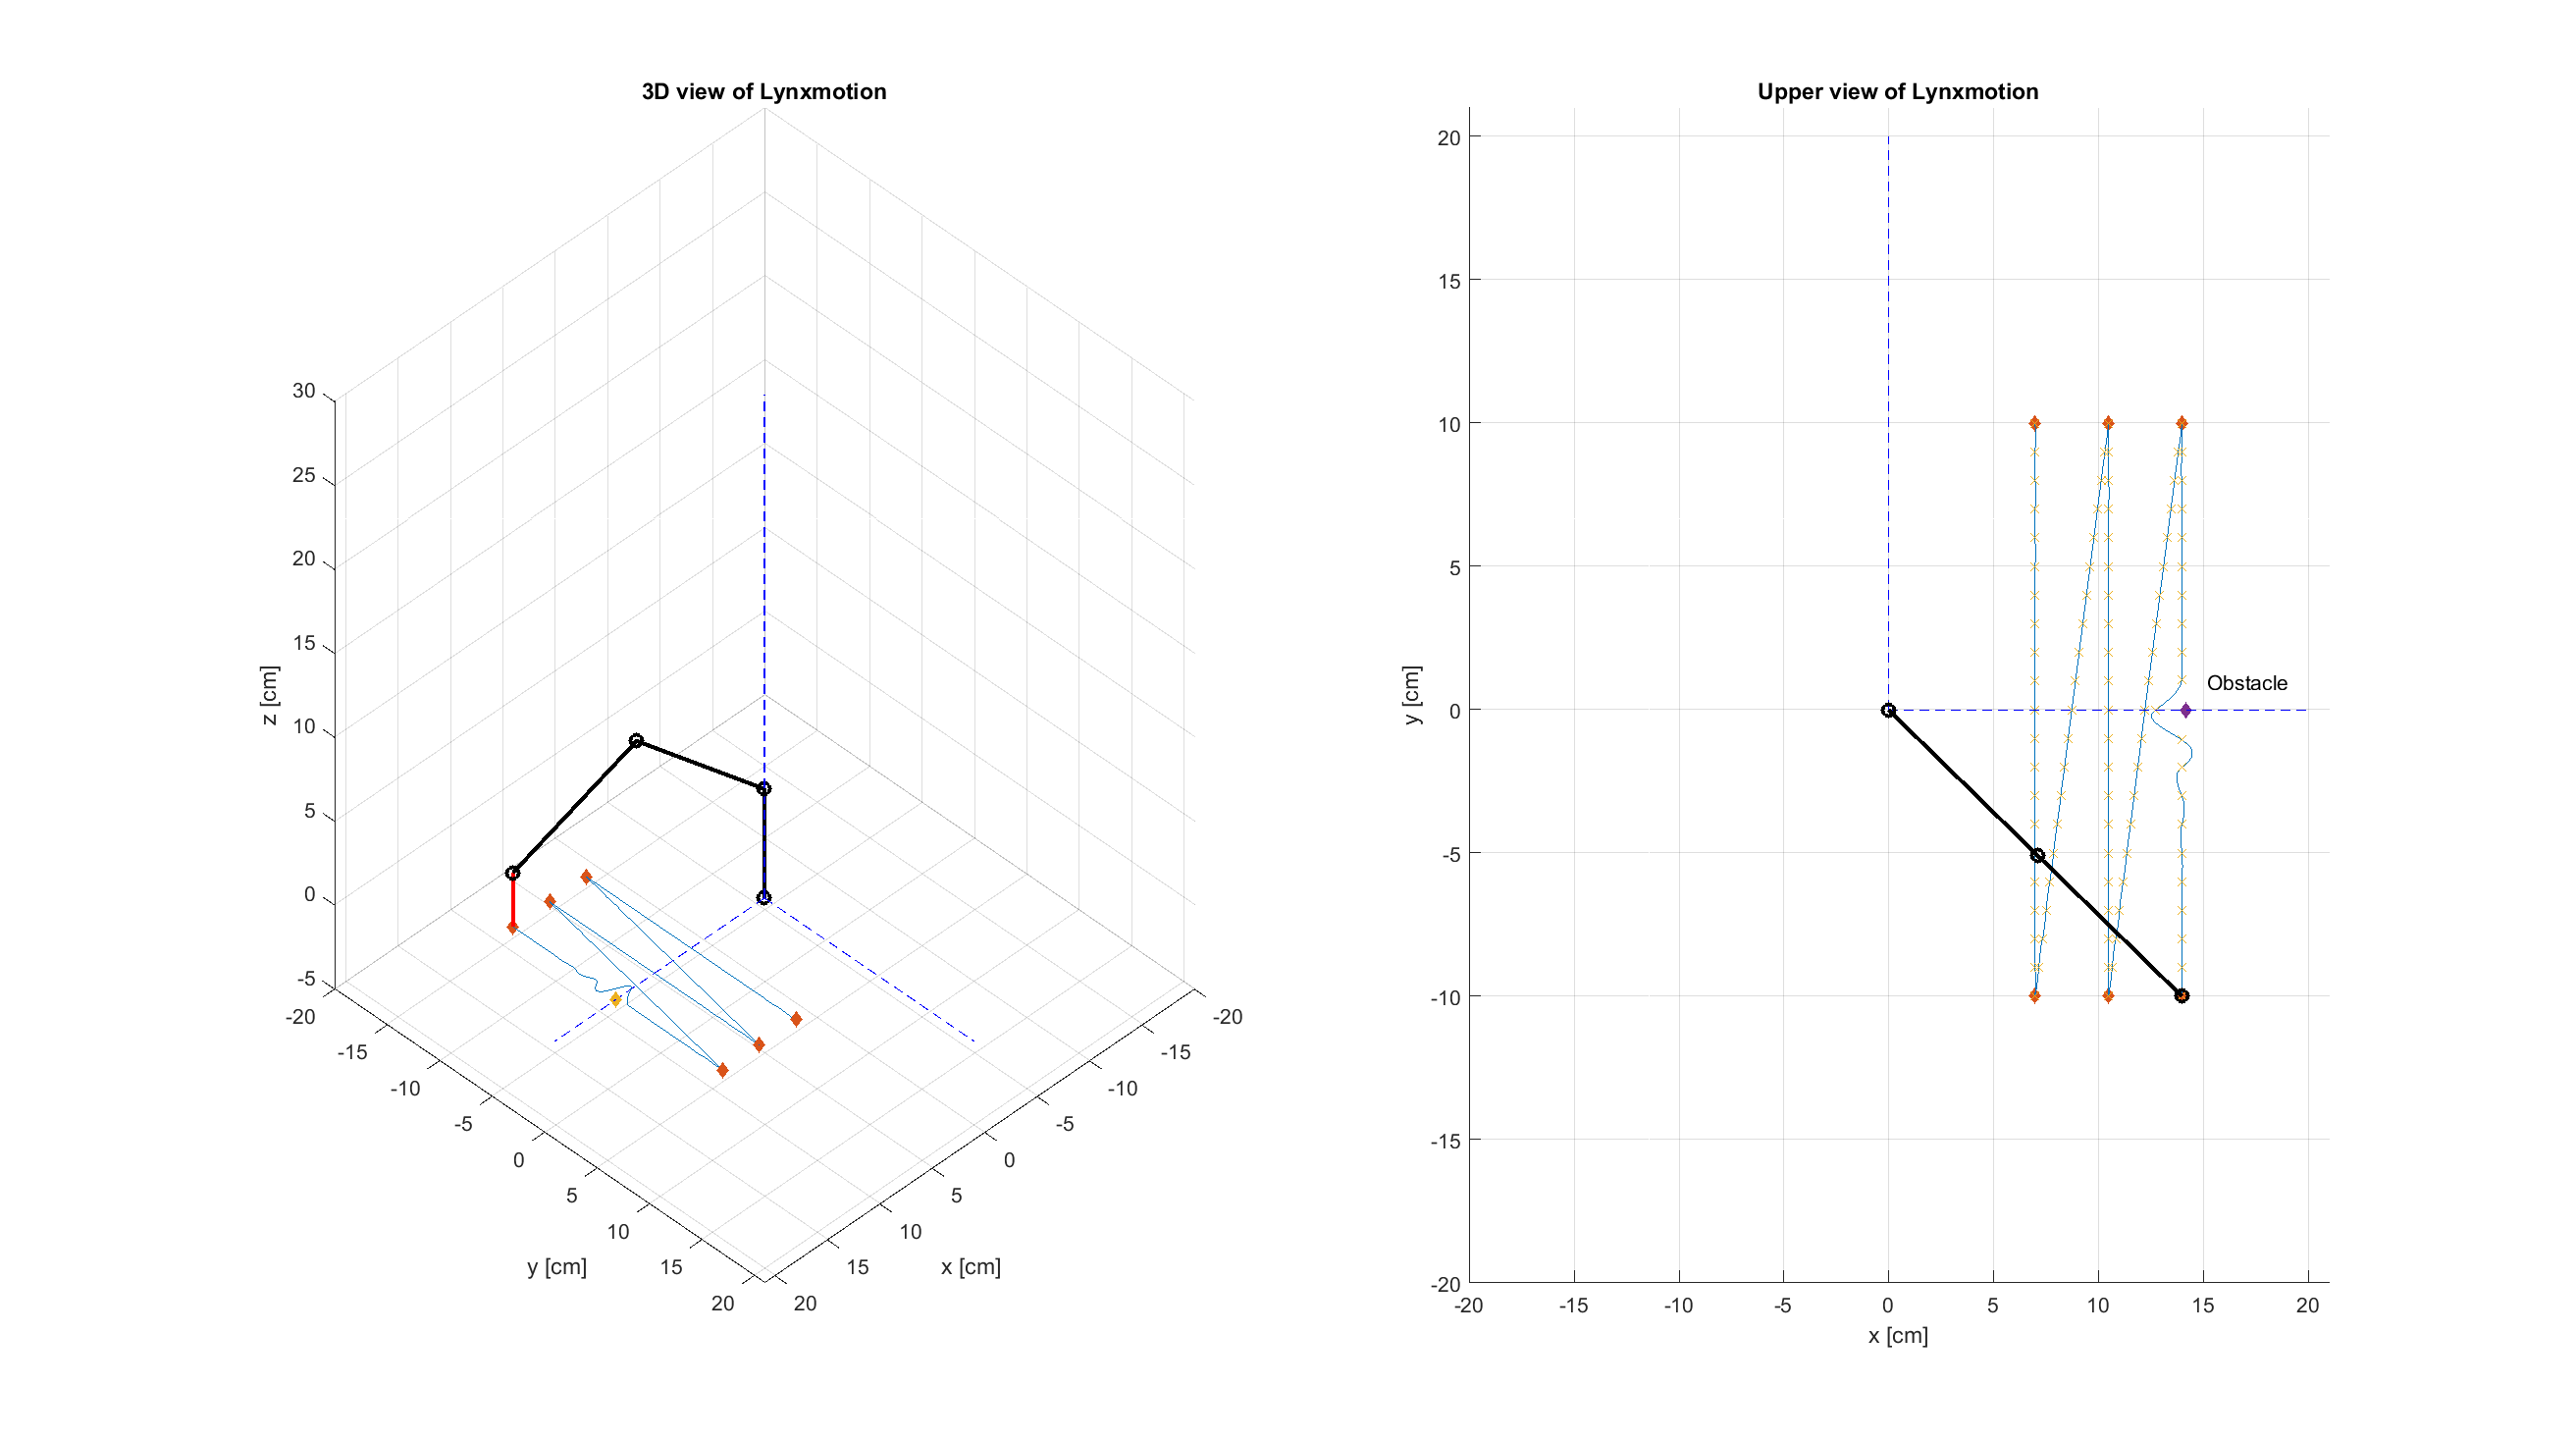
\includegraphics[width=\textwidth]{images/Trajectory_Cartesian}
\caption{Workspace and chosen points}
\label{fig:trajectories.cartesian}
\end{center}
\end{figure}

\section{Part 2}
\subsection{Inverse Kinematics}
The manipilator of this part is a planar parallel robot which applied in surgery. The schematic diagram is shown in  figure \ref{fig:Parallel}. Concretely, The task is to find the solutions for $\psi_i$ and $\theta_i$ given the position coordiante of $C$ with respect to B and the rotation angle $a$ of the platform.
\begin{figure}[htbp] 
\begin{center}
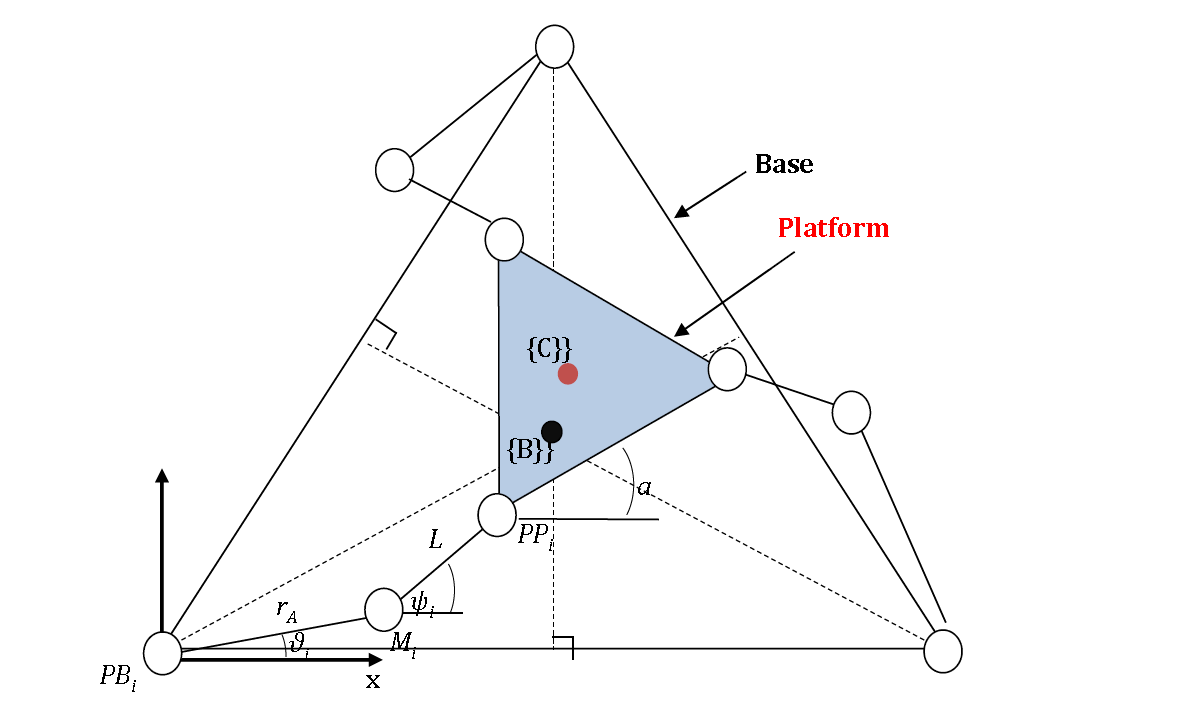
\includegraphics[width=\textwidth]{images/Parallel}
\caption{Planar parallel robot kinematic model}
\label{fig:Parallel}
\end{center}
\end{figure}

The core thinking is that finding the coordinate of $PP_i$ regarding to $PB_i$, which can be derived from the vector  $\overrightarrow{PB_i PP_i}$. According to vector chian, $\overrightarrow{PB_i PP_i}$ can be expressed as

\begin{equation}
\overrightarrow{PB_i PP_i} = \overrightarrow{B PP_i} - \overrightarrow{B PB_i}
\end{equation}

Where, $\overrightarrow{B PB_i}$ is known since ponint $B$ and $PB_i$ is fixed. Then $\overrightarrow{B PP_i}$ can be derived by vector chain again, which is
\begin{equation}
\label{eq:parallel_BPP}
\overrightarrow{B PP_i} = \overrightarrow{BC} + \overrightarrow{C PP_i} = \overrightarrow{BC} + Rot(z,a)\overrightarrow{C_0PP_0} 
\end{equation}
Where $Rot(z,a)$ is the rotation matrix which rorate around $Z$ axis for $a$ degree, $\overrightarrow{C_0PP_0}$ is the initial vector of $\overrightarrow{C PP_i}$ when $a=0$. Therefore, the equation (\ref{eq:parallel_BPP}) can be explicit according to known parameters ($X_c,Y_c$ are the coordinates of $C$,$r_{plat}$ is the radium of platform,$i$ is the number of legs)

\begin{equation}
\overrightarrow{B PP_i} =
\left[\begin{array}{ccc}
	X_c \\
	Y_c \\
	0 \\
\end{array}\right] 
+ \left[\begin{array}{ccc}
	cos(a) & -sin(a) & 0 \\
	sin(a) & cos(a)  & 0 \\
	0      & 0       & 1 \\
\end{array}\right]
\left[\begin{array}{ccc}
	r_{plat}cos(a+pi/2+(i-1)2pi/3) \\
	r_{plat}sin(a+pi/2+(i-1)2pi/3) \\
	0      \\
\end{array}\right]
\end{equation}

Thus, $\overrightarrow{PB_i PP_i}$ can be applied to calculate $\psi_i$ and $\theta_i$ in the $RR$ planar manipulator. Some pure algebra methods are applied subsequently.
For leg $i$ the coordinated for point $PP_i$, w.r.t to frame ${PB}$ are:

\begin{equation}
\label{eq:parallel_x_{ppi}}
x_{pp_i} = r_Acos\theta+Lcos\psi
\end{equation}
\begin{equation}
\label{eq:parallel_y_{ppi}}
y_{pp_i} = r_Asin\theta+Lsin\psi
\end{equation}

Using the above two equations, $(\ref{eq:parallel_x_{ppi}})^2 + (\ref{eq:parallel_y_{ppi}})^2 $, we have
\begin{equation}
\label{eq:parallel_algebra}
x_{pp_i}^2 + y_{pp_i}^2 - 2r_A(x_{pp_i}cos\theta+y_{pp_i}sin\theta)+r_A^2-L^2 = 0
\end{equation}
For simplicity, we define three intermediate parameters to simplify the equation above
\begin{equation}
e_1 = -2y_{pp_i}r_A
\qquad
e_2 = -2x_{pp_i}r_A
\qquad
e_2 =x_{pp_i}^2+y_{pp_i}^2+r_A^2-L^2
\end{equation}

Hence, the euqation \ref{eq:parallel_algebra} can be written as
\begin{equation}
\label{eq:parallel_e}
e_1sin\theta + e_2cos\theta + e_3 = 0
\end{equation}

Then, we define another intermediate parameter $t$ as $t=tan(\frac{\theta}{2})$, we have
\begin{equation}
sin\theta=\frac{2t}{1+t^2}\qquad and \qquad cos\theta=\frac{1-t^2}{1+t^2}
\end{equation}
Substituting them into equation \ref{eq:parallel_e} we derive a quadratic function 
\begin{equation}
(e_3-e_2)t^2+2e_1t+e_2+e_3=0
\end{equation}

The solutions can be solved by a generalized equation
\begin{equation}
\label{eq:parallel_t}
t_{1,2}=\frac{-e_1\pm\sqrt{e_1^2+e_2^2-e_3^2}}{e_3-e_2}
\end{equation}

Therefore, there are 2 solutions for $sin\theta$ and $cos\theta$ individually, namely 2 solutions for $\theta$, they are
\begin{equation}
\theta_1 = atan2(sin\theta_1,cos\theta_1)\qquad and \qquad \theta_2 = atan2(sin\theta_2,cos\theta_2)
\end{equation}

After calculating $\theta$, $\psi$ can be worked out through geometric method as presented in figure \ref{fig:Parallel_psi}
\begin{figure}[htbp] 
\begin{center}
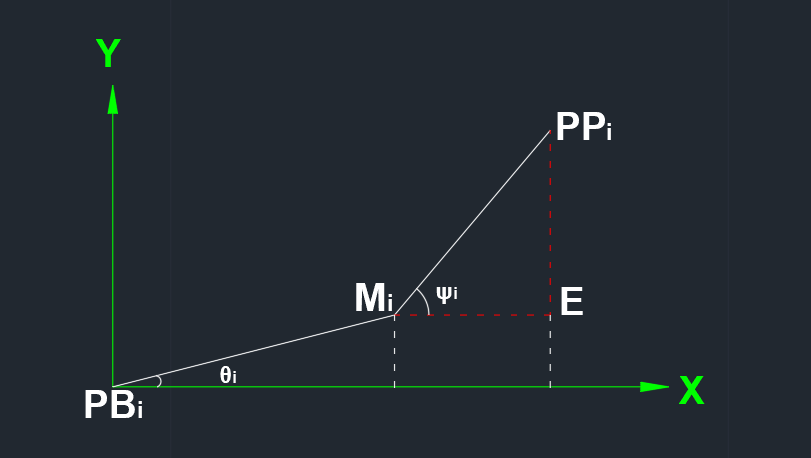
\includegraphics[width=\textwidth]{images/Parallel_psi}
\caption{geometric method for calculating $\psi$}
\label{fig:Parallel_psi}
\end{center}
\end{figure}

\begin{equation}
tan\psi = \frac{PP_iE}{M_iE}=\frac{Y_{PP_i}-r_Asin\theta_i}{X_{PP_i}-r_Acos\theta_i}
\end{equation}

Theoratically, there should be 2 solutions for $\psi$ due the existence of $\theta1$ and $\theta2$, however, the result of $tan\psi$ is the same computed by $\theta1$ and $\theta2$. Therefore, $\psi$ is expressed as
\begin{equation}
\psi = atan2(Y_{PP_i}-r_Asin\theta_i,X_{PP_i}-r_Acos\theta_i )
\end{equation}

\subsection{Workspace}
Algebraic approach relying on the powerful computation of Matlab is a feasible way to calculate the workspace of the end effector. The core thought is that the real root of the equation\ref{eq:parallel_t} exist for each leg when the point is reachable for the manipulator. Namely, three pairs of $t_1,t_2$ for every leg are real number within the workspace. It is a robust method to fit the real workspace by thousands of points forming a region. Then, through specify the coordinate range of point $C$, we can derive the workspace. Concretely, we select a wide range for $X_c,Y_c$ and draw the workspace for different $a$ respectively.
 
\begin{figure}[htbp] 
\begin{center}
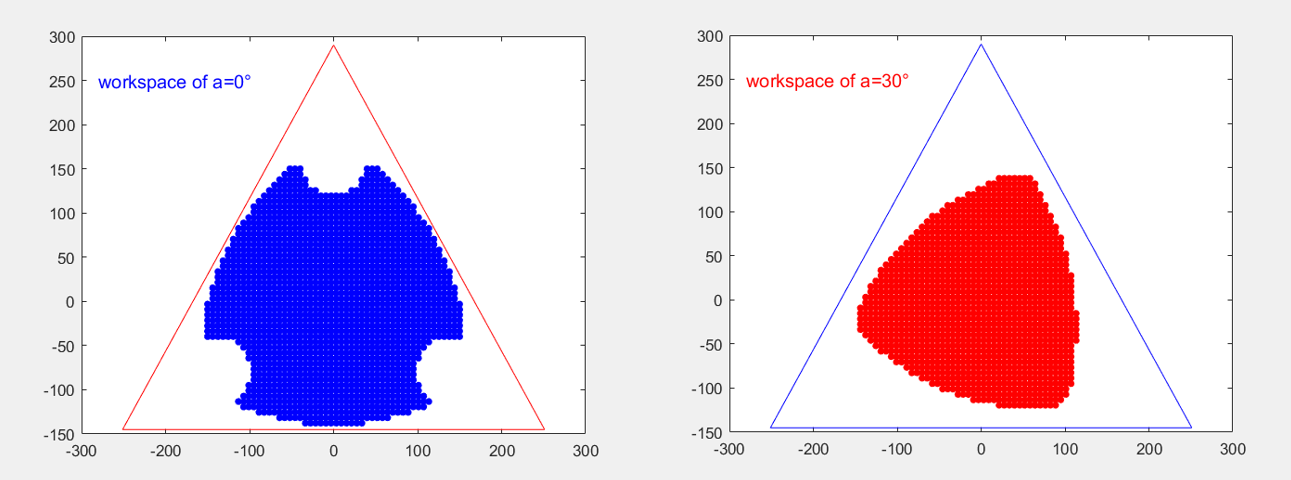
\includegraphics[width=\textwidth]{images/parallel_workspace2}
\caption{Workspace of planar parallel robot when $a=0^{\circ}\qquad a=30^{\circ}$}
\label{fig:parallel_workspace2}
\end{center}
\end{figure}

It is obvious from the picture that different angle $a$ correspond to various shapes of workspace. Furthermore, we find that when $a=0^{\circ}$, the workspace has the biggest shape. It is reasonable as the three legs can stretch themselves to the most in this case. The comparison of different shapes of workspace under diverse angle $a$ is shown in figure \ref{fig:parallel_workspace2}

\begin{figure}[htbp] 
\begin{center}
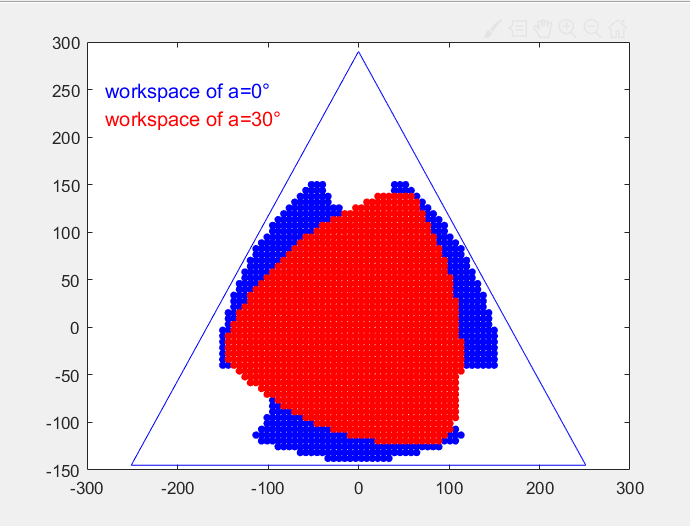
\includegraphics[width=\textwidth]{images/parallel_workspace}
\caption{Comparison of workspace under diverse angle a}
\label{fig:parallel_workspace2}
\end{center}
\end{figure}

\section{Part 3}
\subsection{Rodrigo Moreno Carrillo}
According to \citep{buss2004introduction,barinka2002inverse} there are several methods to solve the inverse kinematics problem. For this part I decided to analyse other approach of solving this problem. The method I decided to evaluate was an iterative method using the pseudo inverse of the Jacobian matrix, similar to the one used in \citep{bhatti2014forward}.

\begin{equation}
x=f(\theta)
\end{equation}

The idea behind this method is that by performing a change in the joint space will bring as a consequence  change in the Cartesian space, this is described by forward kinematics. Therefore if the current configuration is known it is possible to compute the position of the end effector and if the desired position is very close to current position only a slight change in the configuration is needed to achieve that desired position.

\begin{equation}
\label{eq:part3.jacobian_relation}
dx=J(\theta)d\theta
\end{equation}

The relationship between a small change in the joint space and the change in the Cartesian space is given  by (\ref{eq:part3.jacobian_relation}), where $J(\theta)$ is the Jacobian matrix that is defined as:

\begin{equation}
J(\theta)=  \left[
\begin{array}{ccc}
	\frac{\partial f_1}{\partial x_1} & \cdots & \frac{\partial f_1}{\partial x_n} \\
	\vdots & \ddots & \vdots \\
	\frac{\partial f_m}{\partial x_1} & \cdots & \frac{\partial f_m}{\partial x_n} \\
\end{array}
\right] 
\end{equation}

As a consequence, the inverse kinematics problem can be solved by knowing the difference between the current configuration and the configuration that arrives to de desired position, let name it $\Delta\theta$.

\begin{equation}
\theta_d=\theta+\Delta\theta
\end{equation}

If $\Delta\theta$ is considered to be small it can be computed by using inverse jacobian as expressed in (\ref{eq:part3.delta_relation}). Usually as the inverse of jacobian matrix not always exists, it is necessary to use the pseudo-inverse as denoted by \citep{penrose1955generalized}.

\begin{equation}
\label{eq:part3.delta_relation}
\Delta\theta \approx  J(\theta)^{*}\Delta x
\end{equation}

where $J(\theta)^{*}$ is the pseudo-inverse and is computed using (\ref{eq:part3.pseudo_inverse}). The value of $\Delta x$ is the difference or the error between the current position and the desired position 

\begin{equation}
\label{eq:part3.pseudo_inverse}
J(\theta)^{*} = J(\theta)^T(J(\theta)J(\theta)^T)^-1
\end{equation}

Furthermore, a step factor can be added to the equation and completely get the joint values that reduces error and get closer to the desired position.

\begin{figure}[htbp] 
\begin{center}
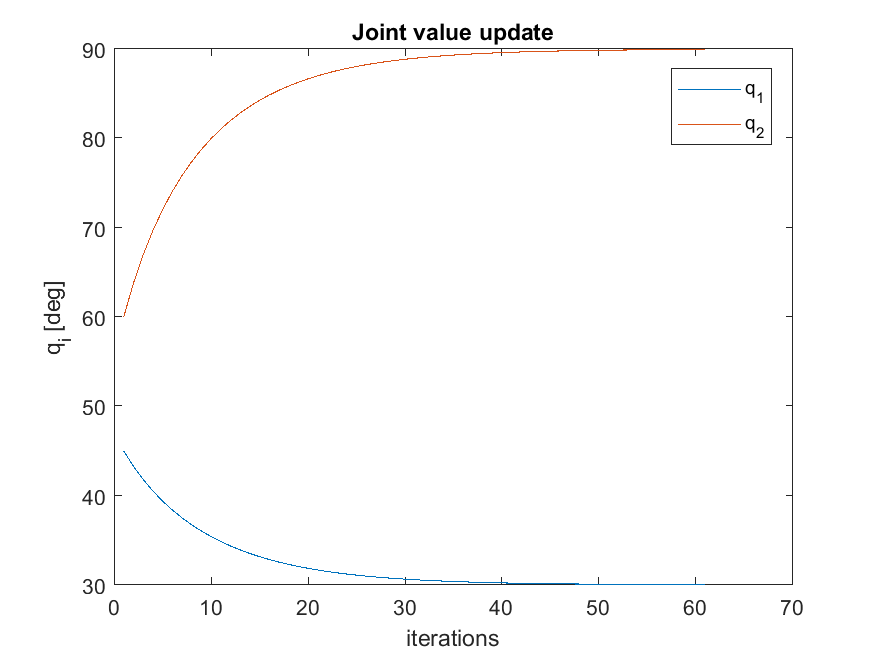
\includegraphics[width=\textwidth]{images/Trajectory_Joint_p3_rodrigo}
\caption{Update process of joint values over the iterations of using the iterative method}
\label{fig:part3.joint_trajectory}
\end{center}
\end{figure}

\begin{equation}
\begin{aligned}
\theta & = \theta + \alpha\Delta\theta \\
& = \theta + \alpha J(\theta)^{*}e \\
&=  \theta + \alpha J(\theta)^{*}(\theta_d - \theta)
\end{aligned}
\end{equation}

Finally, the current joint values are updated using small steps, controlled by $\alpha$, until the error is zero or very close to zero, where can present oscillations  due to the value of $\alpha$ and the precision of the robot.

\begin{figure}[htbp] 
\begin{center}
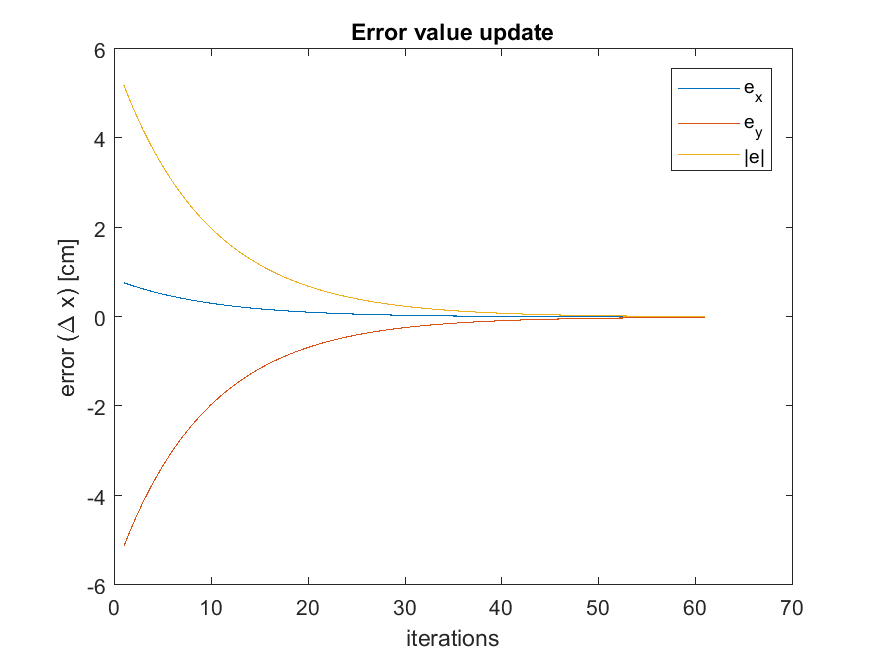
\includegraphics[width=\textwidth]{images/error_p3_rodrigo}
\caption{Error is minimised as the position of end effector gets closer to the desired position}
\label{fig:part3.joint_trajectory}
\end{center}
\end{figure}

For the simulations it was considered a planar robot with two revolute joints, with links of length $a_1=20 [cm]$ and $a_2=10 [cm]$, the coefficient $\alpha = 0.1$. The jacobian of the robot is:

\begin{equation}
J(\theta) = \left[ \begin{array}{cc}
	-a_1\sin(q_1) - a_2\sin(q_1+q_2) & -a_2\sin(q_1+q_2) \\
        a_1\cos(q_1)+a_2\cos(q_1+q_2) & a_2\cos(q_1+q_2) \\
\end{array} \right] 
\end{equation}

The code

\subsection{Mang Ning}












\end{document}
